
%=========================================================
\section{Integrales que producen funciones trigonométricas inversas}
%=========================================================


%=========================================================
\subsection*{Sustitución trigonométrica y reconstrucción mediante
triángulos rectángulos}
%=========================================================

Hasta ahora hemos utilizado cambios de variable en los que una expresión
algebraica se sustituye por una nueva variable. Existe, sin embargo, una
clase de integrales en las que resulta conveniente introducir una función
trigonométrica. A esta técnica se le llama \textbf{sustitución trigonométrica}.

La pregunta natural es: \emph{¿por qué introducir funciones trigonométricas
en una integral que originalmente no contiene ninguna?}

La respuesta está en las identidades pitagóricas. Recordemos

\[
\boxed{
\begin{aligned}
1-\sin^2\theta&=\cos^2\theta,\\
1+\tan^2\theta&=\sec^2\theta,\\
\sec^2\theta-1&=\tan^2\theta.
\end{aligned}}
\]

Estas identidades permiten transformar ciertas sumas o diferencias de
cuadrados en cuadrados perfectos. Ésta es la idea central de la sustitución
trigonométrica.

\subsubsection*{¿Qué problema queremos resolver?}

Las tres estructuras algebraicas que conviene reconocer son

\[
\boxed{a^2-x^2},\qquad
\boxed{a^2+x^2},\qquad
\boxed{x^2-a^2},
\]

frecuentemente dentro de raíces como

\[
\sqrt{a^2-x^2},\qquad
\sqrt{a^2+x^2},\qquad
\sqrt{x^2-a^2}.
\]

La estrategia consiste en elegir una sustitución que convierta la expresión
dentro de la raíz en un cuadrado perfecto. Por ejemplo, si conseguimos que

\[
a^2-x^2=a^2\cos^2\theta,
\]

entonces

\[
\sqrt{a^2-x^2}=\sqrt{a^2\cos^2\theta}=a|\cos\theta|.
\]

Escogiendo adecuadamente el intervalo de valores de $\theta$, podremos
trabajar simplemente con $a\cos\theta$ y habremos eliminado la raíz.

Por tanto, el propósito esencial puede resumirse como

\[
\boxed{\text{convertir una suma o diferencia de cuadrados en un cuadrado perfecto}.}
\]

\subsubsection*{¿Cómo se descubre cada sustitución?}

Para $a^2-x^2$ escribimos

\[
a^2-x^2=a^2\left[1-\left(\frac{x}{a}\right)^2\right].
\]

Al compararla con

\[
1-\sin^2\theta=\cos^2\theta,
\]

resulta natural identificar

\[
\frac{x}{a}=\sin\theta,
\]

y, por tanto,

\[
\boxed{x=a\sin\theta}.
\]

Para $a^2+x^2$ tenemos

\[
a^2+x^2=a^2\left[1+\left(\frac{x}{a}\right)^2\right].
\]

Comparando con

\[
1+\tan^2\theta=\sec^2\theta,
\]

elegimos

\[
\frac{x}{a}=\tan\theta,
\qquad\text{es decir,}\qquad
\boxed{x=a\tan\theta}.
\]

Finalmente,

\[
x^2-a^2=a^2\left[\left(\frac{x}{a}\right)^2-1\right].
\]

La identidad apropiada es

\[
\sec^2\theta-1=\tan^2\theta,
\]

por lo que hacemos

\[
\frac{x}{a}=\sec\theta,
\qquad\text{es decir,}\qquad
\boxed{x=a\sec\theta}.
\]

Así, las sustituciones no son reglas arbitrarias que deban memorizarse de
manera aislada: se deducen comparando la estructura algebraica con una
identidad pitagórica.

\[
\boxed{
\begin{array}{c|c|c}
\text{Expresión} & \text{Identidad} & \text{Sustitución}\\ \hline
 a^2-x^2 & 1-\sin^2\theta=\cos^2\theta & x=a\sin\theta\\[2mm]
 a^2+x^2 & 1+\tan^2\theta=\sec^2\theta & x=a\tan\theta\\[2mm]
 x^2-a^2 & \sec^2\theta-1=\tan^2\theta & x=a\sec\theta
\end{array}}
\]

\subsubsection*{¿Por qué aparece después un triángulo rectángulo?}

La sustitución trigonométrica introduce deliberadamente una nueva variable,
$\theta$. Después de integrar, la respuesta queda expresada en términos de
$\theta$, pero la integral original estaba escrita en términos de $x$.
Debemos, por tanto, regresar a la variable original.

Por ejemplo, si

\[
x=a\sin\theta,
\]

entonces

\[
\sin\theta=\frac{x}{a}.
\]

Como el seno es cateto opuesto entre hipotenusa, podemos construir un
triángulo rectángulo con cateto opuesto $x$ e hipotenusa $a$. Por Pitágoras,
el cateto adyacente es $\sqrt{a^2-x^2}$. De ese único triángulo obtenemos

\[
\sin\theta=\frac{x}{a},\qquad
\cos\theta=\frac{\sqrt{a^2-x^2}}{a},\qquad
\tan\theta=\frac{x}{\sqrt{a^2-x^2}}.
\]

El triángulo no es un adorno: es una herramienta para reconstruir las
funciones trigonométricas de $\theta$ en términos de $x$.

El procedimiento completo puede resumirse así:

\[
\boxed{
\begin{array}{c}
\text{Integral en }x\\
\downarrow\\
\text{Reconocer una suma o diferencia de cuadrados}\\
\downarrow\\
\text{Elegir la identidad pitagórica adecuada}\\
\downarrow\\
\text{Realizar la sustitución trigonométrica}\\
\downarrow\\
\text{Obtener e integrar una expresión en }\theta\\
\downarrow\\
\text{Construir el triángulo rectángulo}\\
\downarrow\\
\text{Regresar de }\theta\text{ a }x
\end{array}}
\]

%---------------------------------------------------------
\subsubsection*{Caso 1: cuando aparece \(\sqrt{a^2-x^2}\)}
%---------------------------------------------------------

Consideremos ahora un ejemplo en el que la sustitución trigonométrica es
realmente necesaria:

\[
I=\int\sqrt{a^2-x^2}\,dx,\qquad a>0.
\]

Como aparece $a^2-x^2$, utilizamos

\[
\boxed{x=a\sin\theta}.
\]

Derivando,

\[
dx=a\cos\theta\,d\theta.
\]

Además,

\begin{align*}
\sqrt{a^2-x^2}
&=\sqrt{a^2-a^2\sin^2\theta}\\
&=a\sqrt{1-\sin^2\theta}\\
&=a\sqrt{\cos^2\theta}\\
&=a|\cos\theta|.
\end{align*}

Aquí aparece un detalle importante. Elegimos

\[
-\frac{\pi}{2}\leq\theta\leq\frac{\pi}{2},
\]

intervalo en el que $\cos\theta\geq0$. Por tanto,

\[
|\cos\theta|=\cos\theta
\]

y podemos escribir

\[
\sqrt{a^2-x^2}=a\cos\theta.
\]

Sustituyendo en la integral,

\begin{align*}
I
&=\int(a\cos\theta)(a\cos\theta\,d\theta)\\
&=a^2\int\cos^2\theta\,d\theta.
\end{align*}

Usamos la identidad de reducción de potencia

\[
\cos^2\theta=\frac{1+\cos(2\theta)}{2}.
\]

Así,

\begin{align*}
I
&=\frac{a^2}{2}\int\left(1+\cos(2\theta)\right)d\theta\\
&=\frac{a^2}{2}\left(\theta+\frac12\sin(2\theta)\right)+C\\
&=\frac{a^2}{2}\theta+
\frac{a^2}{2}\sin\theta\cos\theta+C,
\end{align*}

pues $\sin(2\theta)=2\sin\theta\cos\theta$.

Ahora debemos regresar a $x$. De

\[
x=a\sin\theta
\]

obtenemos

\[
\sin\theta=\frac{x}{a}.
\]

Construimos el triángulo rectángulo correspondiente:

\begin{center}
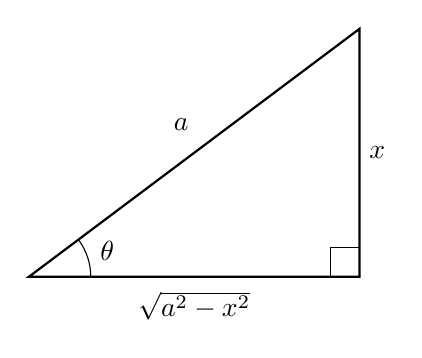
\begin{tikzpicture}[scale=1.05]
    \coordinate (A) at (0,0);
    \coordinate (B) at (4,0);
    \coordinate (C) at (4,3);
    \draw[thick] (A)--(B)--(C)--cycle;
    \draw (3.65,0)--(3.65,0.35)--(4,0.35);
    \node at (2,-0.35) {$\sqrt{a^2-x^2}$};
    \node[right] at (4,1.5) {$x$};
    \node[above left] at (2.05,1.65) {$a$};
    \draw (0.75,0) arc[start angle=0,end angle=36.87,radius=0.75];
    \node at (0.95,0.32) {$\theta$};
\end{tikzpicture}
\end{center}

De él obtenemos

\[
\cos\theta=\frac{\sqrt{a^2-x^2}}{a}
\]

y, por la elección del intervalo principal,

\[
\theta=\arcsin\left(\frac{x}{a}\right).
\]

Sustituyendo,

\begin{align*}
I
&=\frac{a^2}{2}\arcsin\left(\frac{x}{a}\right)
+\frac{a^2}{2}
\left(\frac{x}{a}\right)
\left(\frac{\sqrt{a^2-x^2}}{a}\right)+C\\
&=\frac{x}{2}\sqrt{a^2-x^2}
+\frac{a^2}{2}\arcsin\left(\frac{x}{a}\right)+C.
\end{align*}

Por tanto,

\[
\boxed{
\int\sqrt{a^2-x^2}\,dx
=
\frac{x}{2}\sqrt{a^2-x^2}
+\frac{a^2}{2}\arcsin\left(\frac{x}{a}\right)+C.}
\]

%---------------------------------------------------------
\subsubsection*{Caso 2: cuando aparece \(\sqrt{a^2+x^2}\)}
%---------------------------------------------------------

Consideremos

\[
I=\int\frac{dx}{\sqrt{a^2+x^2}},\qquad a>0.
\]

La suma $a^2+x^2$ sugiere la identidad

\[
1+\tan^2\theta=\sec^2\theta,
\]

por lo que hacemos

\[
\boxed{x=a\tan\theta}.
\]

Entonces

\[
dx=a\sec^2\theta\,d\theta
\]

y

\begin{align*}
\sqrt{a^2+x^2}
&=\sqrt{a^2+a^2\tan^2\theta}\\
&=a\sqrt{1+\tan^2\theta}\\
&=a\sqrt{\sec^2\theta}.
\end{align*}

Tomamos $-\pi/2<\theta<\pi/2$. En este intervalo $\sec\theta>0$, por lo que

\[
\sqrt{a^2+x^2}=a\sec\theta.
\]

Sustituyendo,

\begin{align*}
I
&=\int\frac{a\sec^2\theta}{a\sec\theta}\,d\theta\\
&=\int\sec\theta\,d\theta\\
&=\ln|\sec\theta+\tan\theta|+C.
\end{align*}

Ahora regresamos a $x$. De

\[
\tan\theta=\frac{x}{a}
\]

construimos un triángulo con cateto opuesto $x$ y cateto adyacente $a$.
Por Pitágoras, la hipotenusa es $\sqrt{a^2+x^2}$.

\begin{center}
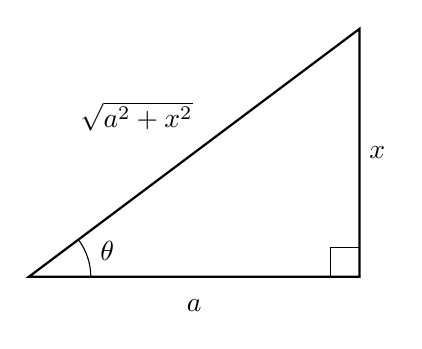
\begin{tikzpicture}[scale=1.05]
    \coordinate (A) at (0,0);
    \coordinate (B) at (4,0);
    \coordinate (C) at (4,3);
    \draw[thick] (A)--(B)--(C)--cycle;
    \draw (3.65,0)--(3.65,0.35)--(4,0.35);
    \node at (2,-0.35) {$a$};
    \node[right] at (4,1.5) {$x$};
    \node[above left] at (2.1,1.65) {$\sqrt{a^2+x^2}$};
    \draw (0.75,0) arc[start angle=0,end angle=36.87,radius=0.75];
    \node at (0.95,0.32) {$\theta$};
\end{tikzpicture}
\end{center}

Así,

\[
\tan\theta=\frac{x}{a},
\qquad
\sec\theta=\frac{\sqrt{a^2+x^2}}{a}.
\]

Por tanto,

\begin{align*}
I
&=\ln\left|
\frac{\sqrt{a^2+x^2}}{a}+\frac{x}{a}
\right|+C\\
&=\ln\left|
\frac{x+\sqrt{a^2+x^2}}{a}
\right|+C.
\end{align*}

Como $a>0$ es constante,

\[
\ln\left|\frac{x+\sqrt{a^2+x^2}}{a}\right|
=\ln|x+\sqrt{a^2+x^2}|-\ln a,
\]

y $-\ln a$ puede absorberse en la constante de integración. Finalmente,

\[
\boxed{
\int\frac{dx}{\sqrt{a^2+x^2}}
=\ln|x+\sqrt{a^2+x^2}|+C.}
\]

%---------------------------------------------------------
\subsubsection*{Caso 3: cuando aparece \(\sqrt{x^2-a^2}\)}
%---------------------------------------------------------

Consideremos ahora

\[
I=\int\frac{dx}{\sqrt{x^2-a^2}},\qquad a>0.
\]

La diferencia $x^2-a^2$ sugiere

\[
\sec^2\theta-1=\tan^2\theta,
\]

por lo que hacemos

\[
\boxed{x=a\sec\theta}.
\]

Derivando,

\[
dx=a\sec\theta\tan\theta\,d\theta.
\]

Además,

\begin{align*}
\sqrt{x^2-a^2}
&=\sqrt{a^2\sec^2\theta-a^2}\\
&=a\sqrt{\sec^2\theta-1}\\
&=a\sqrt{\tan^2\theta}\\
&=a|\tan\theta|.
\end{align*}

Para estudiar, por ejemplo, el caso $x\ge a$, podemos escoger

\[
0\leq\theta<\frac{\pi}{2},
\]

de modo que $\tan\theta\ge0$. Entonces

\[
\sqrt{x^2-a^2}=a\tan\theta.
\]

Sustituyendo,

\begin{align*}
I
&=\int
\frac{a\sec\theta\tan\theta}
     {a\tan\theta}\,d\theta\\
&=\int\sec\theta\,d\theta\\
&=\ln|\sec\theta+\tan\theta|+C.
\end{align*}

De

\[
\sec\theta=\frac{x}{a}
\]

construimos un triángulo rectángulo en el que la hipotenusa es $x$ y el
cateto adyacente es $a$. Por Pitágoras, el cateto opuesto es
$\sqrt{x^2-a^2}$.

\begin{center}
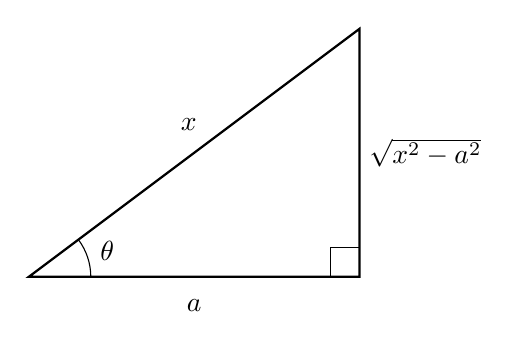
\begin{tikzpicture}[scale=1.05]
    \coordinate (A) at (0,0);
    \coordinate (B) at (4,0);
    \coordinate (C) at (4,3);
    \draw[thick] (A)--(B)--(C)--cycle;
    \draw (3.65,0)--(3.65,0.35)--(4,0.35);
    \node at (2,-0.35) {$a$};
    \node[right] at (4,1.5) {$\sqrt{x^2-a^2}$};
    \node[above left] at (2.15,1.65) {$x$};
    \draw (0.75,0) arc[start angle=0,end angle=36.87,radius=0.75];
    \node at (0.95,0.32) {$\theta$};
\end{tikzpicture}
\end{center}

Así,

\[
\sec\theta=\frac{x}{a},
\qquad
\tan\theta=\frac{\sqrt{x^2-a^2}}{a}.
\]

Por tanto,

\begin{align*}
I
&=\ln\left|
\frac{x}{a}+\frac{\sqrt{x^2-a^2}}{a}
\right|+C\\
&=\ln\left|
\frac{x+\sqrt{x^2-a^2}}{a}
\right|+C.
\end{align*}

Nuevamente, el término constante $-\ln a$ se absorbe en $C$. Así,

\[
\boxed{
\int\frac{dx}{\sqrt{x^2-a^2}}
=\ln|x+\sqrt{x^2-a^2}|+C.}
\]

\subsubsection*{Regla práctica para reconstruir las tres sustituciones}

No es necesario memorizar tres reglas aisladas. Basta recordar las tres
identidades pitagóricas y observar la estructura algebraica:

\[
\boxed{
\begin{array}{c|c|c}
\text{Expresión} & \text{Sustitución} & \text{Relación para el triángulo}\\ \hline
\sqrt{a^2-x^2} & x=a\sin\theta & \displaystyle\sin\theta=\frac{x}{a}\\[3mm]
\sqrt{a^2+x^2} & x=a\tan\theta & \displaystyle\tan\theta=\frac{x}{a}\\[3mm]
\sqrt{x^2-a^2} & x=a\sec\theta & \displaystyle\sec\theta=\frac{x}{a}
\end{array}}
\]

Una forma breve de recordarlo es

\[
\boxed{
\text{resta }a^2-x^2\longrightarrow\sin,
\qquad
\text{suma }a^2+x^2\longrightarrow\tan,
\qquad
\text{resta }x^2-a^2\longrightarrow\sec.}
\]

Lo importante, sin embargo, no es memorizar esta frase sino poder reconstruirla
mediante las identidades pitagóricas.

Faltan ahora las integrales que producen funciones trigonométricas
inversas. Éstas también conviene reconstruirlas a partir de las
derivadas, en vez de memorizarlas sin contexto.

%---------------------------------------------------------
\subsubsection*{Arcoseno}
%---------------------------------------------------------

Sabemos que

\[
\frac{d}{dx}\arcsin x
=
\frac{1}{\sqrt{1-x^2}}.
\]

Leyéndola al revés:

\[
\boxed{
\int\frac{dx}{\sqrt{1-x^2}}
=
\arcsin x+C
}
\]

y, con una constante \(a>0\),

\[
\boxed{
\int\frac{dx}{\sqrt{a^2-x^2}}
=
\arcsin\left(\frac{x}{a}\right)+C
}
\]

porque

\[
\frac{d}{dx}
\arcsin\left(\frac{x}{a}\right)
=
\frac{1/a}{\sqrt{1-x^2/a^2}}
=
\frac{1}{\sqrt{a^2-x^2}}.
\]

%---------------------------------------------------------
\subsubsection*{Arcocoseno}
%---------------------------------------------------------

Como

\[
\frac{d}{dx}\arccos x
=
-\frac{1}{\sqrt{1-x^2}},
\]

tenemos

\[
\boxed{
\int-\frac{dx}{\sqrt{1-x^2}}
=
\arccos x+C
}.
\]

Equivalentemente,

\[
\int\frac{dx}{\sqrt{1-x^2}}
=
-\arccos x+C.
\]

Esto no contradice la fórmula anterior, porque

\[
\arcsin x+\arccos x=\frac{\pi}{2},
\]

de manera que \(\arcsin x\) y \(-\arccos x\) difieren solamente
en una constante.

%---------------------------------------------------------
\subsubsection*{Arcotangente}
%---------------------------------------------------------

Ésta es particularmente importante:

\[
\frac{d}{dx}\arctan x
=
\frac{1}{1+x^2}.
\]

Por tanto,

\[
\boxed{
\int\frac{dx}{1+x^2}
=
\arctan x+C
}.
\]

Para la forma general,

\[
\boxed{
\int\frac{dx}{a^2+x^2}
=
\frac1a\arctan\left(\frac{x}{a}\right)+C,
\qquad a>0.
}
\]

Aquí aparece un factor \(1/a\). Podemos comprobarlo directamente:

\[
\frac{d}{dx}
\left[
\frac1a\arctan\left(\frac{x}{a}\right)
\right]
=
\frac1a
\frac{1/a}{1+x^2/a^2}.
\]

Simplificando,

\[
\frac1a
\frac{1/a}{1+x^2/a^2}
=
\frac{1}{a^2+x^2}.
\]

Por eso,

\[
\boxed{
\int\frac{dx}{x^2+a^2}
=
\frac1a\arctan\left(\frac{x}{a}\right)+C.
}
\]

%---------------------------------------------------------
\subsubsection*{Arcosecante}
%---------------------------------------------------------

Otra forma que suele aparecer en las tablas de integración es

\[
\frac{d}{dx}\operatorname{arcsec}x
=
\frac{1}{|x|\sqrt{x^2-1}}.
\]

Así,

\[
\boxed{
\int
\frac{dx}{|x|\sqrt{x^2-1}}
=
\operatorname{arcsec}x+C
}.
\]

Escalando,

\[
\boxed{
\int
\frac{dx}{|x|\sqrt{x^2-a^2}}
=
\frac1a
\operatorname{arcsec}\left(\frac{|x|}{a}\right)+C
}
\]

con el cuidado correspondiente respecto del dominio y de la
convención empleada para \(\operatorname{arcsec}\).

%---------------------------------------------------------
\subsubsection*{Las dos parejas fundamentales}
%---------------------------------------------------------

Para efectos prácticos, las dos relaciones más importantes son

\[
\boxed{
\begin{aligned}
\frac{d}{dx}\arcsin x
&=\frac{1}{\sqrt{1-x^2}},
&
\int\frac{dx}{\sqrt{1-x^2}}
&=\arcsin x+C,
\\[3mm]
\frac{d}{dx}\arctan x
&=\frac{1}{1+x^2},
&
\int\frac{dx}{1+x^2}
&=\arctan x+C.
\end{aligned}}
\]

De ellas obtenemos las formas escaladas:

\[
\boxed{
\int\frac{dx}{\sqrt{a^2-x^2}}
=
\arcsin\left(\frac{x}{a}\right)+C
}
\]

y

\[
\boxed{
\int\frac{dx}{a^2+x^2}
=
\frac1a\arctan\left(\frac{x}{a}\right)+C.
}
\]

Estas dos formas aparecen constantemente al integrar.

%=========================================================
\subsection*{Deducción mediante funciones trigonométricas inversas}
%=========================================================

Estas fórmulas no tienen por qué memorizarse de manera aislada.
Podemos obtenerlas a partir de las propias funciones trigonométricas
inversas.

\subsubsection*{Deducción para el arco seno}

Sea

\[
y=\arcsin x.
\]

Entonces

\[
x=\sin y.
\]

Derivando implícitamente respecto de \(x\),

\[
1=\cos y\,\frac{dy}{dx}.
\]

Por tanto,

\[
\frac{dy}{dx}
=
\frac1{\cos y}.
\]

Como

\[
\sin y=x,
\]

tenemos

\[
\cos^2y
=
1-\sin^2y
=
1-x^2.
\]

En la rama principal de \(\arcsin\),

\[
-\frac{\pi}{2}\le y\le\frac{\pi}{2},
\]

se tiene \(\cos y\ge0\), por lo que

\[
\cos y=\sqrt{1-x^2}.
\]

Finalmente,

\[
\boxed{
\frac{d}{dx}\arcsin x
=
\frac1{\sqrt{1-x^2}}
}.
\]

Leyendo la derivada al revés,

\[
\boxed{
\int\frac{dx}{\sqrt{1-x^2}}
=
\arcsin x+C.
}
\]

\subsubsection*{Deducción para el arco tangente}

Sea ahora

\[
y=\arctan x.
\]

Entonces

\[
x=\tan y.
\]

Derivando,

\[
1=\sec^2y\,\frac{dy}{dx},
\]

por lo que

\[
\frac{dy}{dx}
=
\frac1{\sec^2y}.
\]

Pero

\[
\sec^2y
=
1+\tan^2y
=
1+x^2.
\]

Entonces

\[
\boxed{
\frac{d}{dx}\arctan x
=
\frac1{1+x^2}
}
\]

y, por tanto,

\[
\boxed{
\int\frac{dx}{1+x^2}
=
\arctan x+C.
}
\]

Así aparecen tres estructuras fundamentales que conviene reconocer:

\[
\boxed{\frac{f'(x)}{f(x)}}
\quad\longrightarrow\quad
\ln|f(x)|,
\]

\[
\boxed{\frac{f'(x)}{\sqrt{1-f(x)^2}}}
\quad\longrightarrow\quad
\arcsin(f(x)),
\]

\[
\boxed{\frac{f'(x)}{1+f(x)^2}}
\quad\longrightarrow\quad
\arctan(f(x)).
\]

